


%\section{Overview}
{\large\textbf{1~~~~Overview}}

The tachometer is intended to interface seamlessly with a 1988 Celebrity Champion power boat. Its primary function is to determine the engine revolutions per minute (RPM) and drive the appropriate gauge to display that RPM. The tachometer is also capable of additional functionality, such as having an LCD screen attached, measuring and displaying oil temperature, coolant temperature, and battery voltage. Additional equipment and documentation is required to enable these additional features.

The tachometer, shown in Figure~\ref{fig:mamad}, is broken into several input/output blocks. Table~\ref{tab:descd} gives information about the labelled portions of Figure~\ref{fig:mamad}.
\begin{figure}[H]
    \centering
    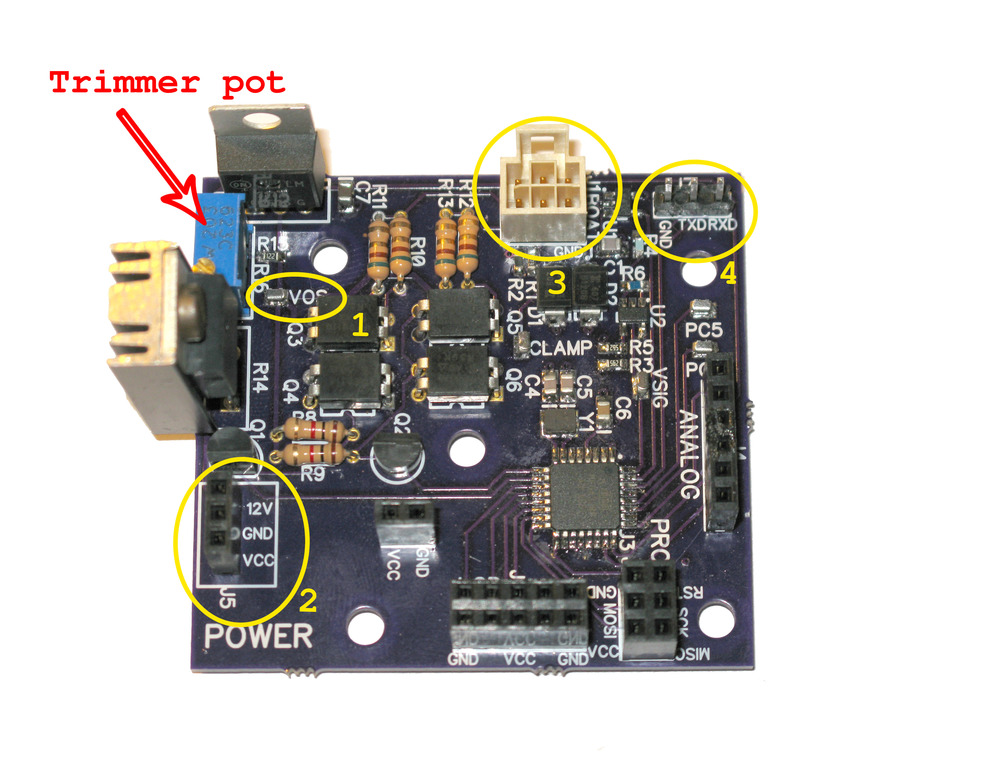
\includegraphics[width=.9\textwidth]{documents/mamaboard}
    \caption{Tachometer}
    \label{fig:mamad}
\end{figure}

% Please add the following required packages to your document preamble:
% \usepackage{booktabs}
\begin{table}[H]
\centering
\caption{Connector descriptions}
\label{tab:descd}
\begin{tabular}{@{}cl@{}}
\toprule
\textbf{Connection} & \textbf{Description} \\ \midrule
1 & Test point for 10V power supply \\
2 & Connector for 5V power supply \\
3 & Connector to boat system \\
4 & Connector for tachometer calibration \\ \bottomrule
\end{tabular}
\end{table}



%\section{Installation}
{\large\textbf{2~~~~Installation}}

Connection~3 is used for interfacing the tachometer to the electrical system on a boat. Figure~\ref{fig:boatcond} shows the pinout.

\begin{figure}[H]
    \centering
    \includegraphics[width=.4\textwidth]{documents/connector}
    \caption{Pinout of Connector 3}
    \label{fig:boatcond}
\end{figure}

The 12V and GND pin connect to the nominal 12V electrical system of a boat and the IGN pin connects to the ignition signal from a gasoline engine. The SIN, COS, and COMM pins connect to the sine, cosine, and common pins of a three-wire  tachometer gauge.

%\section{Calibration}
{\large\textbf{3~~~~Calibration}}

First, the  gauge drive voltage must be set. This can be done by adjusting the trimmer pot shown in Figure~\ref{fig:mamad} until the voltage read at Connection~1 is 10V.

Next, the  gauge operating range and direction must be set, this is done by connecting a 5V logic serial adapter to Connection~4. The tachometer communicates using RS232 at 9600 baud with 8-bit words and one stop bit. After connecting the serial adapter and powering on the tachometer, type CTRL+C on the computer keyboard in a serial console to enter configuration mode. Choose menu option number one, Calibrate tachometer range, to configure the operating range. Press and hold the 1 key until the tachometer needle is at 1000 RPM. The needle should rotate clockwise, if it rotates anti-clockwise, swap the SIN and COS pins on Connector~3. After setting the gauge to 1000 RPM, press enter and hold the 1 key again until the tachometer is at 2000 RPM. Then press enter again to complete calibration.

Menu option two tests the tachometer to confirm a successful calibration without the need to run the engine.

When calibration is done, press the escape key to save the calibration data. The tachometer is ready for use.

%\section{Power Supply}
{\large\textbf{4~~~~Power Supply}}

If the tachometer is not functioning properly, the first thing to check are the power supplies. There are two power supplies on the tachometer, a 10V supply to control the gauge driver circuitry, and a 5V supply for the microcontroller. The 10V supply has a designated test point, Connection 1, labelled \verb|VOS|. If the voltage at \verb|VOS| is not 10V $\pm$100mV, the  trimmer pot can be used to adjust the voltage. If the voltage can not be adjusted to the specified range, the voltage regulator, labelled \verb|U4|, may need replacement. The regulator is an LM317T.

The second power supply attaches to Connection~2. The connector, \verb|J6|, has two pins, a 0V reference and a  5V pin. If the voltage measured across these pins is not 5V, then the power supply may need replacement. A power supply was designed specifically for this project, and may be installed on top tachometer. However, the tachometer is designed such that an off-the-shelf DC-DC converter could be installed should the original fail.

There are many options of DC-DC converter that will work, however it must follow the pinout (shown on main board), and must fit in the provided space. A switching regulator such as the Murata OKI-78SR-5/1.5-W36-C is recommended, though a simple linear regulator such as an LM7805 will also work. If a linear regulator is used, a heat will be required.